\documentclass[11pt,a4paper]{article}
\usepackage[utf8]{inputenc}
\usepackage[T1]{fontenc}
\usepackage{lmodern}
\usepackage[slovak]{babel}
\usepackage[margin=2.5cm]{geometry}
\usepackage{amsmath,amssymb}
\usepackage{graphicx}
\usepackage{booktabs}
\usepackage{tabularx}
\usepackage{array}
\usepackage[hidelinks]{hyperref}

\title{Variant 4A -- Výber akcií alebo indexov}
\author{Lukáš Švihura \and Dominik Keil \and Ján Hrbál}
\date{Moderné prístupy v optimalizácii, zadanie č.\,2, míľnik č.\,2}

\newcolumntype{L}{>{\raggedright\arraybackslash}X}
\setlength{\emergencystretch}{2em}

\begin{document}
\maketitle

% Čísla v texte: results/*.csv a results/examples.txt (scripts/run_baselines.py, scripts/experiment_constraints.py,
% scripts/examples.py). Tabuľka E2: tables/e2.tex (generuje experiment_constraints.py). Tabuľka baseline: tables/baselines.tex (generuje run_baselines.py).

\begin{abstract}
V druhom míľniku sme naprogramovali model úlohy (kandidát, kontrola pravidiel, simulácia
portfólia, Sharpeho pomer), stiahli dáta pre štyri inštancie a model overili na ručne
spočítaných príkladoch a na baseline. Na základe spätnej väzby sme zjednodušili reprezentáciu
kandidáta na jeden vektor podielov, za hlavný baseline berieme \emph{priemer} veľkého počtu
náhodných prípustných portfólií a experimentálne sme porovnali dva spôsoby, ako vynútiť
diverzifikáciu: striktné obmedzenia (oprava kandidáta) a penalizáciu. Bez pravidiel
o počte aktív a veľkosti podielov smeruje maximalizácia Sharpe k portfóliám s 1,4--3,3
efektívnymi aktívami (napr. 83\,\% v jednom dlhopisovom ETF). Striktné obmedzenia dali
pri rovnakom algoritme a rozpočte vždy prípustný výsledok, vyšší Sharpe a výrazne stabilnejšie
behy než penalizácia, preto ich ponechávame. Baseline ukazuje hlavný jav úlohy: optimalizácia
zvýši Sharpe na optimalizačnom období z~0,5--0,9 na 0,9--2,3, ale na testovacom období prekoná
1/N aj priemer náhodných portfólií len v dvoch zo štyroch inštancií.
\end{abstract}

% =====================================================================================
\section{Reakcia na spätnú väzbu k míľniku 1}

Tabuľka~\ref{tab:feedback} zhŕňa pripomienky z opravenej správy a z konzultácie a to, ako sme
ich zapracovali. Podrobnosti sú v uvedených častiach.

\begin{table}[h]
\centering\small
\caption{Pripomienky k míľniku 1 a naša reakcia.}
\label{tab:feedback}
\begin{tabularx}{\textwidth}{@{}p{4.3cm}L@{}}
\toprule
Pripomienka & Reakcia \\
\midrule
Prečo povoľujeme zlomky kusov? &
Ponechávame ich. Pri rozpočte 10\,000\,USD a najmenšom podiele 5\,\% (500\,USD) by sa niektoré
aktíva vôbec nedali kúpiť: akcia Amazonu stála na začiatku roka 2020 približne 1\,900\,USD a
Alphabetu približne 1\,350\,USD (pred neskorším rozdelením akcií). Zlomky kusov dnes ponúka
väčšina brokerov a úloha zostáva spojitá v podieloch (časť~\ref{sec:form}). \\
Dane neuvažujeme. &
Daň závisí od krajiny a doby držby, nie od metódy. Pri jednorazovom nákupe a držbe 2--3 roky
sa týka len konečného zisku a dividend; zníži konečnú sumu všetkých metód podobne a Sharpeho
pomer počas obdobia takmer nemení (priebežne by sa zdaňovali iba dividendy). Ostáva mimo modelu, uvádzame ho medzi obmedzeniami záverov. \\
Načo vektor áno/nie, keď podiel môže byť 0? &
Súhlasíme, vektor bol nadbytočný. Kandidát je teraz jediný vektor podielov $w\in\mathbb{R}^{30}$;
aktívum je vybrané, ak $w_i>0$ (časť~\ref{sec:form}). \\
Nebude optimalizácia smerovať k 100\,\% v najlepšom aktíve? &
Overili sme to (experiment E1, časť~\ref{sec:div}): nie k jednému aktívu, ale k 2--5 aktívam
s jedným dominantným (až 83\,\%). Preto sú pravidlá O3 a O4 potrebné. \\
Sú podiely diskrétne, keď predtým boli z $[0,1]$? &
Podiel je semi-spojitá premenná: $w_i=0$ alebo $w_i\in[0{,}05;\,0{,}30]$. Rozsah $[0,1]$ bol
definičný obor pred uplatnením pravidla O4 (časť~\ref{sec:form}). \\
Argument „10 po 5\,\% a 5 po 30\,\%“ nie je jasný. &
Prepísali sme ho pre každý počet aktív $K$ zvlášť (časť~\ref{sec:form}). \\
Opravovať alebo penalizovať -- ako? &
Opravu aj penalizáciu sme implementovali a popísali (časť~\ref{sec:impl}) a porovnali (E2). \\
Hodnotenie na historických dátach je deterministické? &
Áno. Rovnaký kandidát dostane vždy rovnaké číslo; opravili sme zaradenie (časť~\ref{sec:form}). \\
Ako zabezpečíte platného kandidáta na konci? &
Pri oprave je platný každý ohodnotený kandidát. Pri penalizácii si pamätáme najlepšieho
prípustného a ak žiadny nie je, najlepšieho opravíme. Výstup každej metódy overuje funkcia
\texttt{check} (časť~\ref{sec:impl}). \\
Neberte najlepšieho, ale priemer z veľa náhodných. &
Hlavný baseline je priemer 10\,000 náhodných prípustných portfólií. Náhodné prehľadávanie
(najlepší z~5\,000) ponechávame len ako referenciu pre algoritmy a uvádzame priemer
a odchýlku cez 20 behov (časť~\ref{sec:base}). \\
Zohľadniť mieru diverzifikácie bez ohľadu na výnos? &
Zaviedli sme efektívny počet aktív $N_\text{eff}=1/\sum_i w_i^2$, uvádzame ho pri každom
výsledku a vyskúšali sme ho ako penalizáciu (E2). \\
Penalizovať nízku diverzifikáciu (napr. portfólio z~1--2 aktív), alebo použiť pevné limity? &
Porovnali sme oboje na ladiacej inštancii. Vyhrali pevné limity (časť~\ref{sec:div}). \\
\bottomrule
\end{tabularx}
\end{table}

% =====================================================================================
\section{Upresnená formulácia}
\label{sec:form}

\paragraph{Kandidát.} Vektor podielov $w=(w_1,\dots,w_n)$, $n=30$. Množina vybraných aktív je
$S(w)=\{i: w_i>0\}$. Pri nákupe v prvý deň obdobia $t_0$ dostaneme $w_i B/P_i(t_0)$ kusov
aktíva $i$ ($B=10\,000$\,USD), takže hodnota portfólia je
\[
  V(t) \;=\; B\sum_{i\in S(w)} w_i\,\frac{P_i(t)}{P_i(t_0)} .
\]
Podiely sa počas držby menia podľa vývoja cien (portfólio nevyvažujeme).

\paragraph{Ohodnocovacia funkcia} (maximalizujeme): Sharpeho pomer denných výnosov
$r(t)=V(t)/V(t-1)-1$ na optimalizačnom období, $f(w)=\bar r/s_r\cdot\sqrt{252}$, bez bezrizikovej sadzby.

\paragraph{Obmedzenia.}
\begin{align*}
 &\text{(O1)}\ \textstyle\sum_i w_i = 1, &
 &\text{(O2, O4)}\ w_i\in\{0\}\cup[\ell,u],\quad \ell=0{,}05,\ u=0{,}30, \\
 &\text{(O5)}\ w_i=0 \text{ pre aktíva bez cien,} &
 &\text{(O3)}\ k_{\min}\le|S(w)|\le k_{\max},\quad k_{\min}=5,\ k_{\max}=10.
\end{align*}
Pravidlo O5 sa vzťahuje na optimalizačné obdobie (to investor v čase rozhodnutia pozná).
Premenná $w_i$ je teda \emph{semi-spojitá}: buď presne 0, alebo spojitá hodnota z~$[\ell,u]$.
Úloha je kombinatorická vo výbere $S$ a spojitá v podieloch vybraných aktív.

\paragraph{Poplatky, dividendy a dane.} Transakčné poplatky nezapočítavame (zdôvodnenie
v~míľniku~1: mnohí brokeri obchodujú akcie a ETF bez poplatku a pri jednorazovom nákupe a
predaji by znížili výsledok všetkých metód takmer rovnako). Dividendy sú zahrnuté v~upravených
cenách, teda ako okamžite reinvestované do toho istého aktíva. Dane neuvažujeme.

\paragraph{Prečo prípustné riešenia vždy existujú.} Ak vyberieme $K$ aktív a každé má podiel
v~$[\ell,u]$, ich súčet môže byť ľubovoľné číslo z~$[K\ell,\,Ku]$. Pravidlo O1 sa dá splniť
práve vtedy, keď $K\ell\le 1\le Ku$, teda $1/u\le K\le 1/\ell$, čo je $3{,}33\le K\le 20$.
Napríklad pre $K=5$ je súčet z~$[25\,\%;\,150\,\%]$ a pre $K=10$ z~$[50\,\%;\,300\,\%]$;
100\,\% leží v oboch. Každý povolený počet $K\in\{5,\dots,10\}$ preto leží v tomto rozsahu a
\emph{ľubovoľný} výber 5 až 10 aktív sa dá doplniť na prípustné portfólio. Práve to využíva
oprava v časti~\ref{sec:impl}.

\paragraph{Diverzifikácia, ktorú pravidlá zaručujú.} Mieru diverzifikácie nezávislú od výnosov
meriame efektívnym počtom aktív $N_\text{eff}=1/\sum_i w_i^2$ (inverzný Herfindahlov index):
$K$ rovnakých podielov dá $K$, jedno aktívum dá~1. Najmenšie $N_\text{eff}$, ktoré pravidlá
O1--O4 pripúšťajú, má portfólio $3\times 30\,\% + 2\times 5\,\%$, a to
$1/(3\cdot 0{,}09+2\cdot 0{,}0025)=3{,}64$.

\paragraph{Oprava zaradenia (determinizmus).} Ohodnocovacia funkcia je deterministická:
rovnaký kandidát na rovnakých historických dátach dostane vždy rovnaké číslo, a to na
optimalizačnom aj testovacom období. Náhodná je len skutočná budúcnosť, ktorú historické
dáta iba odhadujú. Preto výsledok overujeme na testovacom období, ktoré algoritmus nevidí.
Ostatné zaradenia z~míľnika~1 sa nemenia.

% =====================================================================================
\section{Dáta a inštancie}
\label{sec:data}

Denné záverečné ceny sme stiahli z~Yahoo Finance (knižnica \texttt{yfinance}, ceny upravené
o~dividendy a delenia akcií) za roky 2010--2025 a uložili do \texttt{data/prices.csv}, aby boli
experimenty reprodukovateľné. Kontrolovali sme medzery a extrémne denné zmeny: jediné zmeny
nad 25\,\% sú skutočné pohyby akcie Meta (2013, 2022). Odčlenenia firiem (GE~2023, AT\&T~2022)
sú v~upravených cenách zahrnuté, nespôsobujú skoky.

Každá inštancia má 15 rovnakých ETF a 15 akcií, ktoré boli najväčšími americkými firmami podľa
trhovej kapitalizácie ku koncu roka pred začiatkom optimalizačného obdobia
(tabuľka~\ref{tab:inst}). ETF: SPY, IWM (akcie USA), VGK (Európa), EWJ (Japonsko),
EEM (rozvíjajúce sa trhy), AGG, TLT, LQD (dlhopisy), GLD (zlato), VNQ (nehnuteľnosti)
a sektory XLK, XLE, XLV, XLF, XLP. Všetky aktíva majú vo všetkých inštanciách ceny počas celého
obdobia, pravidlo O5 teda žiadne aktívum nevylučuje (je však implementované).

Ladiaca inštancia používa len dáta do roku 2017, kým všetky testovacie obdobia hodnotiacich
inštancií začínajú v~roku 2018. Ladenie metód a rozhodnutia o formulácii preto nevidia žiadne
dáta, na ktorých metódy záverečne hodnotíme.

\begin{table}[h]
\centering\small
\caption{Inštancie. Ladiacu používame len na nastavenie metód a rozhodnutia o formulácii.}
\label{tab:inst}
\begin{tabularx}{\textwidth}{@{}lllL@{}}
\toprule
Inštancia & Optimalizácia & Test & Akcie (15 najväčších firiem k~31.\,12. roka pred optimalizáciou) \\
\midrule
ladiaca & 2011--2014 & 2015--2017 & XOM, AAPL, MSFT, BRK-B, GE, WMT, GOOGL, CVX, IBM, PG, JNJ, T, JPM, WFC, KO \\
I1 & 2014--2017 & 2018--2020 & AAPL, XOM, GOOGL, MSFT, BRK-B, GE, JNJ, WMT, CVX, WFC, JPM, PG, IBM, VZ, PFE \\
I2 & 2017--2020 & 2021--2023 & AAPL, GOOGL, MSFT, BRK-B, AMZN, XOM, META, JNJ, JPM, WFC, GE, T, PG, BAC, CVX \\
I3 & 2020--2023 & 2024--2025 & AAPL, MSFT, GOOGL, AMZN, META, BRK-B, JPM, V, JNJ, WMT, BAC, PG, MA, XOM, T \\
\bottomrule
\end{tabularx}
\end{table}

% =====================================================================================
\section{Implementácia modelu}
\label{sec:impl}

Kód je v Pythone (\texttt{numpy}, \texttt{pandas}, \texttt{scipy}), spúšťanie popisuje
\texttt{README.md}.

\begin{itemize}
\item \texttt{instance.py} -- trieda \texttt{Instance}: názvy aktív, matice cien
  (dni $\times$ aktíva) pre optimalizačné a testovacie obdobie, príznak dostupnosti (O5)
  a parametre pravidiel $B,k_{\min},k_{\max},\ell,u$. Metóda \texttt{with\_rules} vytvorí
  kópiu s inými pravidlami (pre neskoršie zväčšenie úlohy).
\item \texttt{model.py} -- \texttt{check(w, inst)} vráti zoznam porušených pravidiel
  (napr. \texttt{O3 počet aktív 2 mimo [5, 10]}), \texttt{evaluate} spočíta Sharpe, ročný
  výnos, ročné kolísanie, najväčší prepad, konečnú hodnotu a $N_\text{eff}$.
  Trieda \texttt{Evaluator} je rýchla ohodnocovacia funkcia s~počítadlom ohodnotení: ceny
  vydelí cenami v deň nákupu raz vopred, takže jedno ohodnotenie je jedno násobenie matice
  $1006\times 30$ vektorom a trvá rádovo desiatky mikrosekúnd (22--57\,µs podľa počítača). Počítadlo použijeme na férové porovnanie metód.
\item \texttt{repair.py} -- oprava, dekóder skóre a penalizačné funkcie (nižšie).
\item \texttt{baselines.py} -- baseline a referenčné prehľadávania (časť~\ref{sec:base}).
\end{itemize}

\paragraph{Oprava (repair).} Ľubovoľný vektor $v\in\mathbb{R}^{30}$ zmení na prípustné portfólio:
\begin{enumerate}
\item záporné zložky a nedostupné aktíva nastaví na 0 (O2, O5);
\item ak je nenulových zložiek viac ako $k_{\max}$, ponechá $k_{\max}$ najväčších; ak menej ako
  $k_{\min}$, doplní aktíva s najvyššou prioritou (pri dekóderi skóre), inak náhodné (O3);
\item zložky vybraných aktív nahradí \emph{najbližším} bodom (v euklidovskej vzdialenosti) so súčtom 1
  a zložkami v~$[\ell,u]$ (O1, O4).
\end{enumerate}
Najbližší bod v kroku 3 má tvar $w_i=\min(u,\max(\ell, v_i-\tau))$ (podmienky optimality
Karusha--Kuhna--Tuckera). Súčet je v~$\tau$ nerastúca po častiach lineárna funkcia so zlommi
v bodoch $v_i-u$ a $v_i-\ell$, preto $\tau$ nájdeme presne: zoradíme zlomy, nájdeme úsek,
v ktorom súčet prechádza cez 1, a dopočítame lineárnou interpoláciou. Pre $K$ medzi 5 a 10 je
krok 3 podľa časti~\ref{sec:form} vždy riešiteľný, takže výsledok je vždy prípustný.
Už prípustný vektor oprava nezmení. Príklad: podiely 25/25/25/20/3/2\,\% (dva pod 5\,\%)
oprava zmení na 23,8/23,8/23,8/18,8/5/5\,\% -- malé podiely zvýši na 5\,\% a rozdiel rovnomerne
uberie ostatným.

\paragraph{Dekóder skóre} (reprezentácia cez skóre z míľnika 1). Jedinec je 30 čísel z~$[0,1]$;
vybrané sú aktíva so skóre nad 0,5, ich počet sa oreže alebo doplní podľa skóre na
$[k_{\min},k_{\max}]$ a skóre vybraných aktív sa opravou premietnu na podiely. Z každého vektora
skóre vznikne prípustné portfólio deterministicky (rovnaké skóre $\to$ rovnaké portfólio);
dekódovanie trvá 25--65\,µs podľa počítača. Vlastnosť, ktorú treba poznať: pri rovnomerne
náhodných skóre je nad prahom v~priemere 15 aktív, takže dekóder v~približne 98\,\% prípadov
vyberie presne $k_{\max}=10$ aktív. Náhodná štartovacia populácia (napr. pri diferenciálnej
evolúcii) preto obsahuje takmer len portfóliá s~10 aktívami; menší počet aktív musí algoritmus
nájsť sám (lokálne prehľadávanie sa dostane aj na 5 aktív, časť~\ref{sec:div}).

\paragraph{Penalizácia.} Kandidát sa iba normalizuje (záporné na 0, súčet na 1, teda O1 a O2
platia vždy) a ohodnotenie je $f(w)-\lambda\, p(w)$. Implementovali sme dve miery porušenia:
\begin{itemize}
\item \emph{pravidlá}: $p(w)=\max(0,k_{\min}-|S|)+\max(0,|S|-k_{\max})+\frac{1}{0{,}05}\sum_{i\in S}
  \bigl(\max(0,\ell-w_i)+\max(0,w_i-u)\bigr)$ -- jedno chýbajúce aktívum alebo 5 p.\,b. mimo
  hraníc podielu je jedna jednotka;
\item \emph{diverzifikácia} (návrh z konzultácie): $p(w)=\max(0,\,5-N_\text{eff}(w))+\frac{1}{0{,}05}\sum_i\max(0,w_i-u)$
  -- portfólio s~1--2 aktívami je penalizované, rozumne rozložené nie, bez ohľadu na výnosy.
\end{itemize}
Penalizovaný algoritmus si pamätá najlepšieho \emph{prípustného} kandidáta, ktorého počas behu
ohodnotil, a ten aj vráti; ak žiadneho nenašiel, najlepšieho podľa penalizovanej funkcie opraví.
Tak má na konci vždy platného kandidáta.

% =====================================================================================
\section{Overenie modelu}
\label{sec:verify}

\paragraph{Unit testy} (\texttt{tests/test\_model.py}, 24 testov, všetky prechádzajú) overujú model
na príkladoch spočítaných ručne. Napríklad: aktívum A stojí 100, 110, 99\,USD a aktívum B
50, 50, 60\,USD; portfólio 50/50 z~1\,000\,USD kúpi 5 kusov A a 10 kusov B, takže hodnoty sú
1\,000, 1\,050 a 1\,095\,USD a denné výnosy 5\,\% a 4,29\,\% -- model vráti presne tieto hodnoty
aj zodpovedajúci Sharpe. Ďalšie testy overujú najväčší prepad
($100\to120\to90$ je prepad 25\,\%), že rýchly \texttt{Evaluator} dáva to isté ako úplná
simulácia, že dve aktíva s opačným kolísaním majú spolu vyšší Sharpe ako každé zvlášť, že
\texttt{check} odhalí porušenie každého pravidla O1--O5 a že oprava, dekóder aj generátor
náhodných portfólií dajú na 2\,000 náhodných vstupoch vždy prípustný výsledok. Presný výpočet
projekcie porovnávame s bisekciou na 500 náhodných vstupoch. Generátor náhodných portfólií
overujeme aj pri prísnejších pravidlách ($u=20\,\%$, keď sa pri $K=5$ dá súčet 1 splniť len
rovnakými podielmi) a pri nesplniteľných pravidlách, ktoré musia skončiť chybou.

\paragraph{Príklady na skutočných dátach} (inštancia I1, \texttt{scripts/examples.py},
tabuľka~\ref{tab:examples}). Kandidát B (100\,\% Microsoft, akcia s~najvyšším Sharpe na optimalizačnom
období) a C~(dve akcie) majú vysoký Sharpe, ale \texttt{check} ich správne odmietne. Kandidát D
porušuje len O4, oprava ho posunie na prípustné portfólio s~takmer rovnakým hodnotením.
Kandidát~E (1/N všetkých 30) porušuje O3 aj O4.

\begin{table}[h]
\centering\small
\caption{Ohodnotenie vybraných kandidátov na inštancii I1 (optimalizácia 2014--2017, test 2018--2020).}
\label{tab:examples}
\begin{tabularx}{\textwidth}{@{}lLlrrrr@{}}
\toprule
 & Portfólio & Kontrola & Sharpe opt. & Sharpe test & Konečná suma test & $N_\text{eff}$ \\
\midrule
A & SPY 30, VGK 20, GLD 15, MSFT 20, JNJ 15\,\% & prípustné & 1,14 & 0,87 & 16\,031 & 4,65 \\
B & MSFT 100\,\% & O3, O4 & 1,19 & 1,19 & 26\,998 & 1,00 \\
C & MSFT 60, AAPL 40\,\% & O3, O4 & 1,29 & 1,29 & 29\,006 & 1,92 \\
D & SPY, TLT, GLD po 25, JNJ 20, AAPL 3, MSFT 2\,\% & O4 & 1,46 & 1,21 & 14\,547 & 4,37 \\
E & 30 aktív po 3,33\,\% & O3, O4 & 0,99 & 0,59 & 13\,171 & 30,00 \\
\bottomrule
\end{tabularx}
\end{table}

% =====================================================================================
\section{Diverzifikácia: striktné obmedzenia alebo penalizácia?}
\label{sec:div}

\paragraph{E1: Kam smeruje maximalizácia Sharpe bez pravidiel O3, O4?} Na optimalizačnom období
každej inštancie sme numericky riešili úlohu len s O1 a O2 (nelineárny solver SLSQP z~\texttt{scipy},
20 náhodných štartov). Solver nájde lokálne optimum a Sharpe pri držbe bez vyvažovania nemusí mať
jediné optimum, preto výsledok berieme ako najlepšiu nájdenú hodnotu. Výsledok (tabuľka~\ref{tab:e1}) nie je 100\,\% v najlepšom aktíve:
kombinácia aktív má vždy vyšší Sharpe než najlepšie samostatné aktívum (napr. 2,05 oproti 1,23
v I1), lebo kolísania sa čiastočne rušia. Je však silne koncentrovaný: $N_\text{eff}$ je len 1,4--3,3
a najväčší podiel 48--83\,\%, najmä v~dlhopisoch a zlate, ktoré v daných obdobiach málo kolísali.
Keďže pravidlá O3 a O4 prípustnú množinu len zmenšujú, slúži táto hodnota zároveň ako
orientačný horný odhad pre našu úlohu s~obmedzeniami; žiadna z~metód ho neprekročila.

\begin{table}[h]
\centering\small
\caption{E1: maximalizácia Sharpe na optimalizačnom období bez pravidiel O3 a O4.}
\label{tab:e1}
\setlength{\tabcolsep}{4pt}
\begin{tabular}{@{}llrrrrl@{}}
\toprule
Inšt. & Najlepšie 1 aktívum & Sharpe & Aktív & $N_\text{eff}$ & Max. & Hlavné zložky \\
\midrule
ladiaca & XLV (1,51) & 2,36 & 9 & 2,71 & 56\,\% & AGG 56, XLV 17, TLT 13, XLP 8\,\% \\
I1 & XLK (1,23) & 2,05 & 5 & 1,44 & 83\,\% & AGG 83, JPM 8, JNJ 4, MSFT 3\,\% \\
I2 & AAPL (1,40) & 1,83 & 7 & 3,25 & 48\,\% & TLT 48, GLD 23, AAPL 11, PG 6\,\% \\
I3 & AAPL (0,89) & 0,95 & 4 & 3,02 & 48\,\% & GLD 48, AAPL 22, MSFT 20, XOM 10\,\% \\
\bottomrule
\end{tabular}
\end{table}

\paragraph{E2: striktné obmedzenia vs. penalizácia.} Na ladiacej inštancii sme spustili
\emph{ten istý} algoritmus -- (1+1) lokálne prehľadávanie v priestore skóre $[0,1]^{30}$
(gaussovská mutácia, v priemere 2 zmenené zložky, $\sigma=0{,}1$) -- s rozpočtom 5\,000 ohodnotení
a 20 behmi. Varianty sa líšia len tým, ako sa zo skóre stane hodnotené portfólio:
dekóder s opravou (striktné obmedzenia, aj s prísnejším $u=20\,\%$), normalizácia bez O3, O4,
penalizácia pravidiel pre tri hodnoty $\lambda$ a penalizácia nízkej diverzifikácie
($N_\text{eff}<5$). Rozhodnutie robíme len na ladiacej inštancii, aby výber formulácie nevidel
dáta inštancií zo záverečného porovnania.

\begin{table}[h]
\centering\small
\caption{E2: rovnaký algoritmus s rôznou prácou s obmedzeniami (ladiaca inštancia, 20 behov
$\times$ 5\,000 ohodnotení). „Prípustné“ = podiel behov, ktorých najlepší kandidát podľa vlastnej
funkcie spĺňa O1--O5; „neprípustné ohodn.“ = podiel ohodnotení minutých na neprípustných
kandidátov. $N_\text{eff}$ a Sharpe sú pre odovzdané (vždy prípustné) portfólio, Sharpe ako
priemer $\pm$ smer. odchýlka.}
\label{tab:e2}
\begin{tabular}{@{}lrrrrr@{}}
\toprule
Variant & Prípustné & Nepríp. ohodn. & $N_\text{eff}$ & Sharpe opt. & Sharpe test \\
\midrule
striktné (oprava) & 100\,\% & 0{,}0\,\% & 4{,}26 & 2{,}34\,$\pm$\,0{,}001 & 0{,}92\,$\pm$\,0{,}021\\
striktné, max. podiel 20\,\% & 100\,\% & 0{,}0\,\% & 5{,}78 & 2{,}31\,$\pm$\,0{,}011 & 1{,}01\,$\pm$\,0{,}032\\
bez O3/O4 & 0\,\% & 68{,}3\,\% & 3{,}66 & 2{,}23\,$\pm$\,0{,}128 & 0{,}87\,$\pm$\,0{,}058\\
penalizácia pravidiel $\lambda=$0{,}01 & 90\,\% & 18{,}6\,\% & 4{,}47 & 2{,}23\,$\pm$\,0{,}129 & 0{,}87\,$\pm$\,0{,}048\\
penalizácia pravidiel $\lambda=$0{,}1 & 100\,\% & 7{,}9\,\% & 4{,}70 & 2{,}27\,$\pm$\,0{,}037 & 0{,}88\,$\pm$\,0{,}076\\
penalizácia pravidiel $\lambda=$1 & 100\,\% & 6{,}4\,\% & 4{,}70 & 2{,}27\,$\pm$\,0{,}037 & 0{,}88\,$\pm$\,0{,}076\\
penalizácia $N_\text{eff}<5$ $\lambda=$0{,}1 & 100\,\% & 4{,}1\,\% & 5{,}02 & 2{,}26\,$\pm$\,0{,}011 & 0{,}89\,$\pm$\,0{,}042\\
penalizácia $N_\text{eff}<5$ $\lambda=$1 & 100\,\% & 3{,}7\,\% & 5{,}55 & 2{,}24\,$\pm$\,0{,}011 & 0{,}97\,$\pm$\,0{,}055\\
\bottomrule
\end{tabular}

\end{table}

Výsledky (tabuľka~\ref{tab:e2}):
\begin{itemize}
\item \textbf{Striktné obmedzenia} dali vo všetkých behoch prípustný výsledok, žiadne ohodnotenie
  sa neminulo na neprípustného kandidáta a dosiahli najvyšší Sharpe na optimalizačnom období
  (2,34, len o 1\,\% menej ako orientačný horný odhad 2,36 z~E1) s~veľmi malým rozptylom medzi behmi.
  Prísnejší strop $u=20\,\%$ vynúti rozloženejšie portfóliá ($N_\text{eff}=5{,}8$) za cenu
  1\,\% Sharpe na optimalizačnom období a stále bez jediného neprípustného ohodnotenia.
\item \textbf{Penalizácia pravidiel} závisí od $\lambda$: pri $\lambda=0{,}01$ je výhodnejšie
  pravidlo porušiť a 10\,\% behov skončilo s neprípustným najlepším kandidátom. Pri vyšších
  $\lambda$ sú výsledky prípustné, ale 6--8\,\% ohodnotení padne na neprípustných kandidátov a
  priemerný Sharpe je nižší (2,27) s~rádovo väčším rozptylom (smerodajná odchýlka 0,037 oproti
  0,002). Penalizácia vytvára na hranici prípustnej oblasti strmé „útesy“, cez ktoré lokálne
  prehľadávanie ťažko prechádza. Výsledky pre $\lambda=0{,}1$ a $\lambda=1$ sú rovnaké: už pri
  $\lambda=0{,}1$ je pokuta za porušenie väčšia než zisk Sharpe, ktorý by porušenie prinieslo,
  preto obe hodnoty dovedú behy k~rovnakým portfóliám a líšia sa len podielom neprípustných
  ohodnotení počas behu.
\item \textbf{Penalizácia diverzifikácie} ($N_\text{eff}<5$) viedla k~rozloženejším portfóliám
  ($N_\text{eff}$ 5,0--5,6 oproti 4,3) s~mierne nižším Sharpe na optimalizačnom období. Na
  testovacom období bol pri $\lambda=1$ vyšší (0,97 oproti 0,92), pri $\lambda=0{,}1$ mierne
  nižší (0,89). Rovnaký efekt, ešte o niečo silnejší (test 1,01), však dosiahol aj striktný
  strop 20\,\% bez penalizácie a bez neprípustných ohodnotení. Lepší test teda súvisí so
  silnejšou diverzifikáciou, nie s penalizáciou ako takou. Ide o jedno testovacie obdobie a
  rozdiely sú menšie ako rozptyl náhodných portfólií (časť~\ref{sec:base}), preto z~nich
  nerobíme silný záver.
\end{itemize}

\paragraph{Rozhodnutie.} Ponechávame \textbf{striktné obmedzenia} O3, O4, zabudované priamo do
reprezentácie (dekóder/oprava), ako sme sa dohodli na konzultácii („minimum a maximum do reprezentácie“).
Dôvody: (1) výsledok je vždy prípustný a nemusíme dokazovať, že penalizácia na konci „dotiahne“
kandidáta do prípustnej oblasti; (2) netreba ladiť $\lambda$, ktorej vhodná hodnota závisí od
rozsahu Sharpeho pomeru v inštancii; (3) celý rozpočet ohodnotení ide na prípustných kandidátov;
(4) pravidlá typu „najviac $x$\,\% v jednom aktíve“ sú v praxi tvrdé limity (napr. pravidlá pre
investičné fondy), nie odporúčania. Diverzifikácia je tak zaručená ($N_\text{eff}\ge 3{,}64$);
$N_\text{eff}$ ďalej uvádzame pri každom výsledku. Silu diverzifikácie riadime parametrami
pravidiel ($k_{\min}$, $u$), nie penalizáciou. V~míľniku 3 preto porovnáme metódy pri
$u=30\,\%$ aj $u=20\,\%$; o tom, ktorú hodnotu použijeme ako hlavnú, rozhodneme
na ladiacej inštancii. Penalizáciu ponecháme v kóde ako alternatívu na porovnanie.

% =====================================================================================
\section{Baseline}
\label{sec:base}

\begin{itemize}
\item \textbf{Náhodné prípustné portfóliá -- priemer} (hlavný baseline podľa spätnej väzby).
  Počet aktív $K$ náhodne z~5--10, $K$ náhodných aktív a podiely
  $w_i=\ell+(1-K\ell)\,d_i$, kde $d\sim\text{Dirichlet}(1,\dots,1)$ je rovnomerne náhodný bod
  simplexu; kandidátov s niektorým $w_i>u$ zamietneme a losujeme znova. Takto je každý kandidát
  prípustný bez opravy a podiely sú pre daný výber aktív rozdelené rovnomerne na celej prípustnej
  množine (oprava by naopak hromadila podiely na hraniciach 5 a 30\,\%). Uvádzame priemer a
  smerodajnú odchýlku cez 10\,000 portfólií. Ukazuje, čo dosiahne investor, ktorý pravidlá dodrží,
  ale nič neoptimalizuje -- a aký veľký je rozptyl samotnej náhody.
\item \textbf{10 náhodných aktív po 10\,\%} (baseline z míľnika 1), tiež priemer cez 10\,000.
\item \textbf{Greedy top-10}: 10 aktív s najvyšším vlastným Sharpe na optimalizačnom období po
  10\,\%. Odpovedá na otázku, čo dá „investovať do najlepších aktív podľa Sharpe“ bez ohľadu
  na to, ako sa navzájom dopĺňajú.
\item \textbf{Náhodné prehľadávanie} (najlepší z~5\,000 náhodných prípustných) a \textbf{(1+1) lokálne
  prehľadávanie} s dekóderom (ako v~E2), oba s~5\,000 ohodnoteniami a 20 behmi. Nie sú to
  baseline v zmysle spätnej väzby, ale referencie pre algoritmy z~míľnika~3 pri rovnakom
  rozpočte: navrhnutá metóda musí byť lepšia aspoň od nich.
\item \textbf{1/N všetkých 30 aktív} -- porušuje O3, uvádzame ho len ako známu ťažko
  prekonateľnú referenciu pre test \cite{demiguel2009}.
\end{itemize}

\begin{table}[h]
\centering\small
\caption{Baseline a referencie. Sharpe na optimalizačnom (opt.) a testovacom období; ostatné
stĺpce na testovacom období: ročný výnos, ročné kolísanie, najväčší prepad (v \%) a konečná suma
z 10\,000\,USD. Pri priemeroch je pri teste uvedená smerodajná odchýlka cez portfóliá/behy.}
\label{tab:base}
\setlength{\tabcolsep}{4pt}
\begin{tabular}{@{}lrrrrrrr@{}}
\toprule
Metóda & Sharpe opt. & Sharpe test & $N_\text{eff}$ & Výnos & Kolísanie & Prepad & Suma \\
\midrule
\multicolumn{8}{@{}l}{\textbf{ladiaca}}\\
náhodné prípustné (priemer) & 0{,}94 & 0{,}85\,$\pm$\,0{,}21 & 6{,}28 & 9{,}3 & 11{,}3 & 13{,}7 & 13\,085\\
10 náhodných po 10\,\% (priemer) & 0{,}96 & 0{,}88\,$\pm$\,0{,}16 & 10{,}00 & 9{,}4 & 10{,}8 & 12{,}9 & 13\,088\\
greedy top-10 Sharpe & 1{,}46 & 1{,}09 & 10{,}00 & 10{,}2 & 9{,}4 & 10{,}9 & 13\,389\\
náhodné prehľadávanie (5\,000 ohodn.) & 1{,}95 & 0{,}95\,$\pm$\,0{,}17 & 5{,}14 & 6{,}8 & 7{,}2 & 9{,}2 & 12\,187\\
lokálne prehľadávanie (5\,000 ohodn.) & 2{,}34 & 0{,}93\,$\pm$\,0{,}05 & 4{,}30 & 5{,}6 & 6{,}1 & 8{,}3 & 11\,776\\
1/N všetkých 30 (mimo O3) & 0{,}98 & 0{,}93 & 30{,}00 & 9{,}4 & 10{,}3 & 11{,}8 & 13\,082\\
\midrule
\multicolumn{8}{@{}l}{\textbf{I1}}\\
náhodné prípustné (priemer) & 0{,}91 & 0{,}56\,$\pm$\,0{,}25 & 6{,}28 & 9{,}4 & 19{,}8 & 28{,}7 & 13\,206\\
10 náhodných po 10\,\% (priemer) & 0{,}94 & 0{,}57\,$\pm$\,0{,}19 & 10{,}00 & 9{,}4 & 19{,}3 & 28{,}4 & 13\,150\\
greedy top-10 Sharpe & 1{,}41 & 0{,}96 & 10{,}00 & 19{,}1 & 20{,}4 & 26{,}7 & 16\,883\\
náhodné prehľadávanie (5\,000 ohodn.) & 1{,}70 & 1{,}11\,$\pm$\,0{,}13 & 5{,}10 & 14{,}6 & 12{,}9 & 17{,}5 & 15\,091\\
lokálne prehľadávanie (5\,000 ohodn.) & 1{,}96 & 1{,}30\,$\pm$\,0{,}03 & 5{,}13 & 12{,}9 & 9{,}7 & 14{,}9 & 14\,399\\
1/N všetkých 30 (mimo O3) & 0{,}99 & 0{,}59 & 30{,}00 & 9{,}6 & 18{,}6 & 28{,}0 & 13\,171\\
\midrule
\multicolumn{8}{@{}l}{\textbf{I2}}\\
náhodné prípustné (priemer) & 0{,}78 & 0{,}69\,$\pm$\,0{,}22 & 6{,}28 & 10{,}9 & 16{,}6 & 22{,}7 & 13\,681\\
10 náhodných po 10\,\% (priemer) & 0{,}80 & 0{,}73\,$\pm$\,0{,}17 & 10{,}00 & 11{,}0 & 15{,}9 & 21{,}2 & 13\,706\\
greedy top-10 Sharpe & 1{,}35 & 0{,}56 & 10{,}00 & 8{,}4 & 17{,}0 & 28{,}3 & 12\,736\\
náhodné prehľadávanie (5\,000 ohodn.) & 1{,}54 & 0{,}17\,$\pm$\,0{,}18 & 4{,}89 & 1{,}5 & 12{,}8 & 24{,}5 & 10\,481\\
lokálne prehľadávanie (5\,000 ohodn.) & 1{,}80 & $-$0{,}07\,$\pm$\,0{,}01 & 4{,}76 & $-$1{,}1 & 10{,}0 & 22{,}5 & 9\,661\\
1/N všetkých 30 (mimo O3) & 0{,}84 & 0{,}78 & 30{,}00 & 11{,}1 & 15{,}0 & 19{,}6 & 13\,692\\
\midrule
\multicolumn{8}{@{}l}{\textbf{I3}}\\
náhodné prípustné (priemer) & 0{,}53 & 1{,}45\,$\pm$\,0{,}31 & 6{,}28 & 20{,}3 & 13{,}4 & 14{,}4 & 14\,479\\
10 náhodných po 10\,\% (priemer) & 0{,}55 & 1{,}54\,$\pm$\,0{,}24 & 10{,}00 & 20{,}4 & 12{,}6 & 14{,}0 & 14\,475\\
greedy top-10 Sharpe & 0{,}81 & 1{,}60 & 10{,}00 & 23{,}1 & 13{,}6 & 14{,}2 & 15\,124\\
náhodné prehľadávanie (5\,000 ohodn.) & 0{,}86 & 1{,}75\,$\pm$\,0{,}24 & 4{,}85 & 24{,}9 & 13{,}3 & 13{,}9 & 15\,561\\
lokálne prehľadávanie (5\,000 ohodn.) & 0{,}94 & 1{,}77\,$\pm$\,0{,}03 & 4{,}10 & 25{,}5 & 13{,}3 & 12{,}5 & 15\,712\\
1/N všetkých 30 (mimo O3) & 0{,}57 & 1{,}64 & 30{,}00 & 20{,}4 & 11{,}8 & 13{,}8 & 14\,476\\
\bottomrule
\end{tabular}

\end{table}

\begin{figure}[h]
\centering
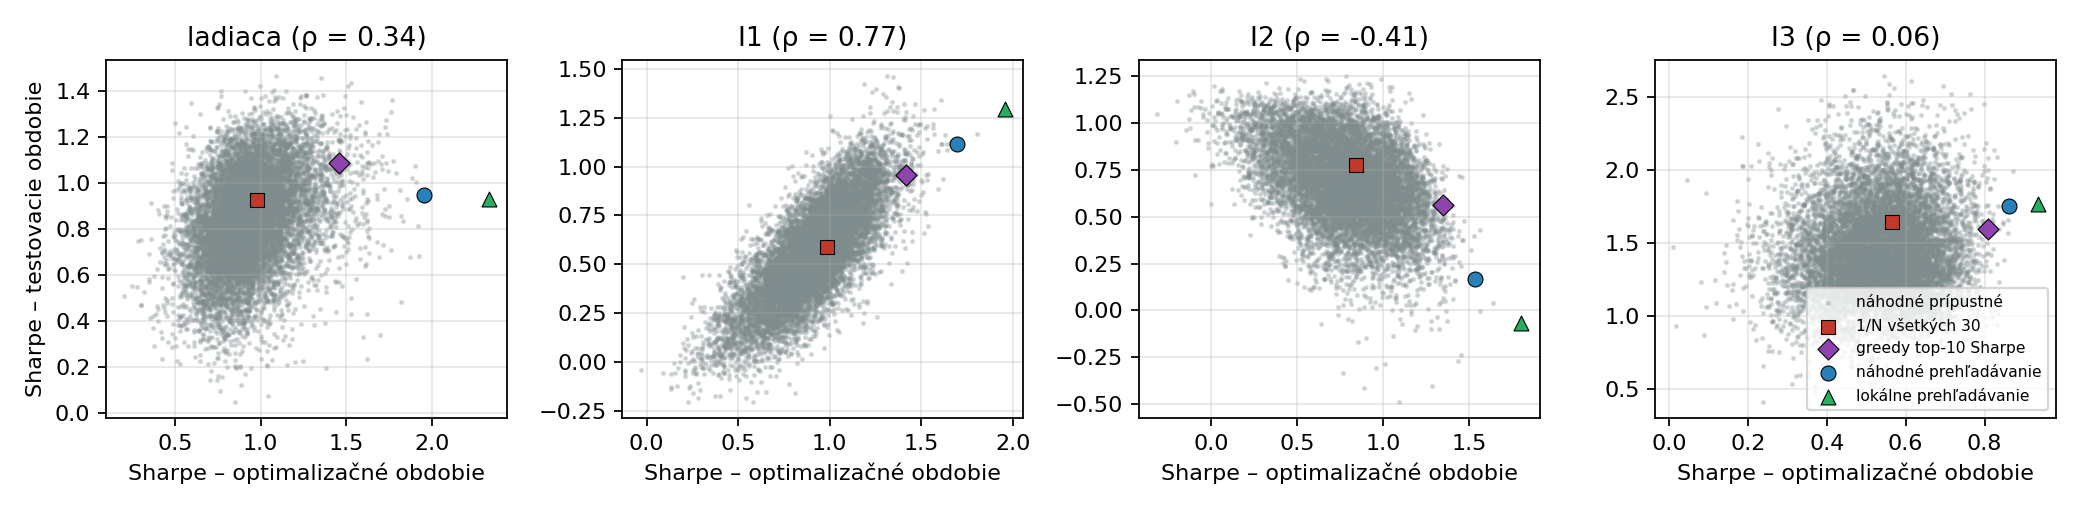
\includegraphics[width=0.8\textwidth]{figures/random_train_test.png}
\caption{Sharpe 10\,000 náhodných prípustných portfólií na optimalizačnom (os $x$) a testovacom
(os $y$) období a poloha referenčných metód. $\rho$ je Spearmanova korelácia medzi oboma
obdobiami.}
\label{fig:random}
\end{figure}

\begin{figure}[h]
\centering
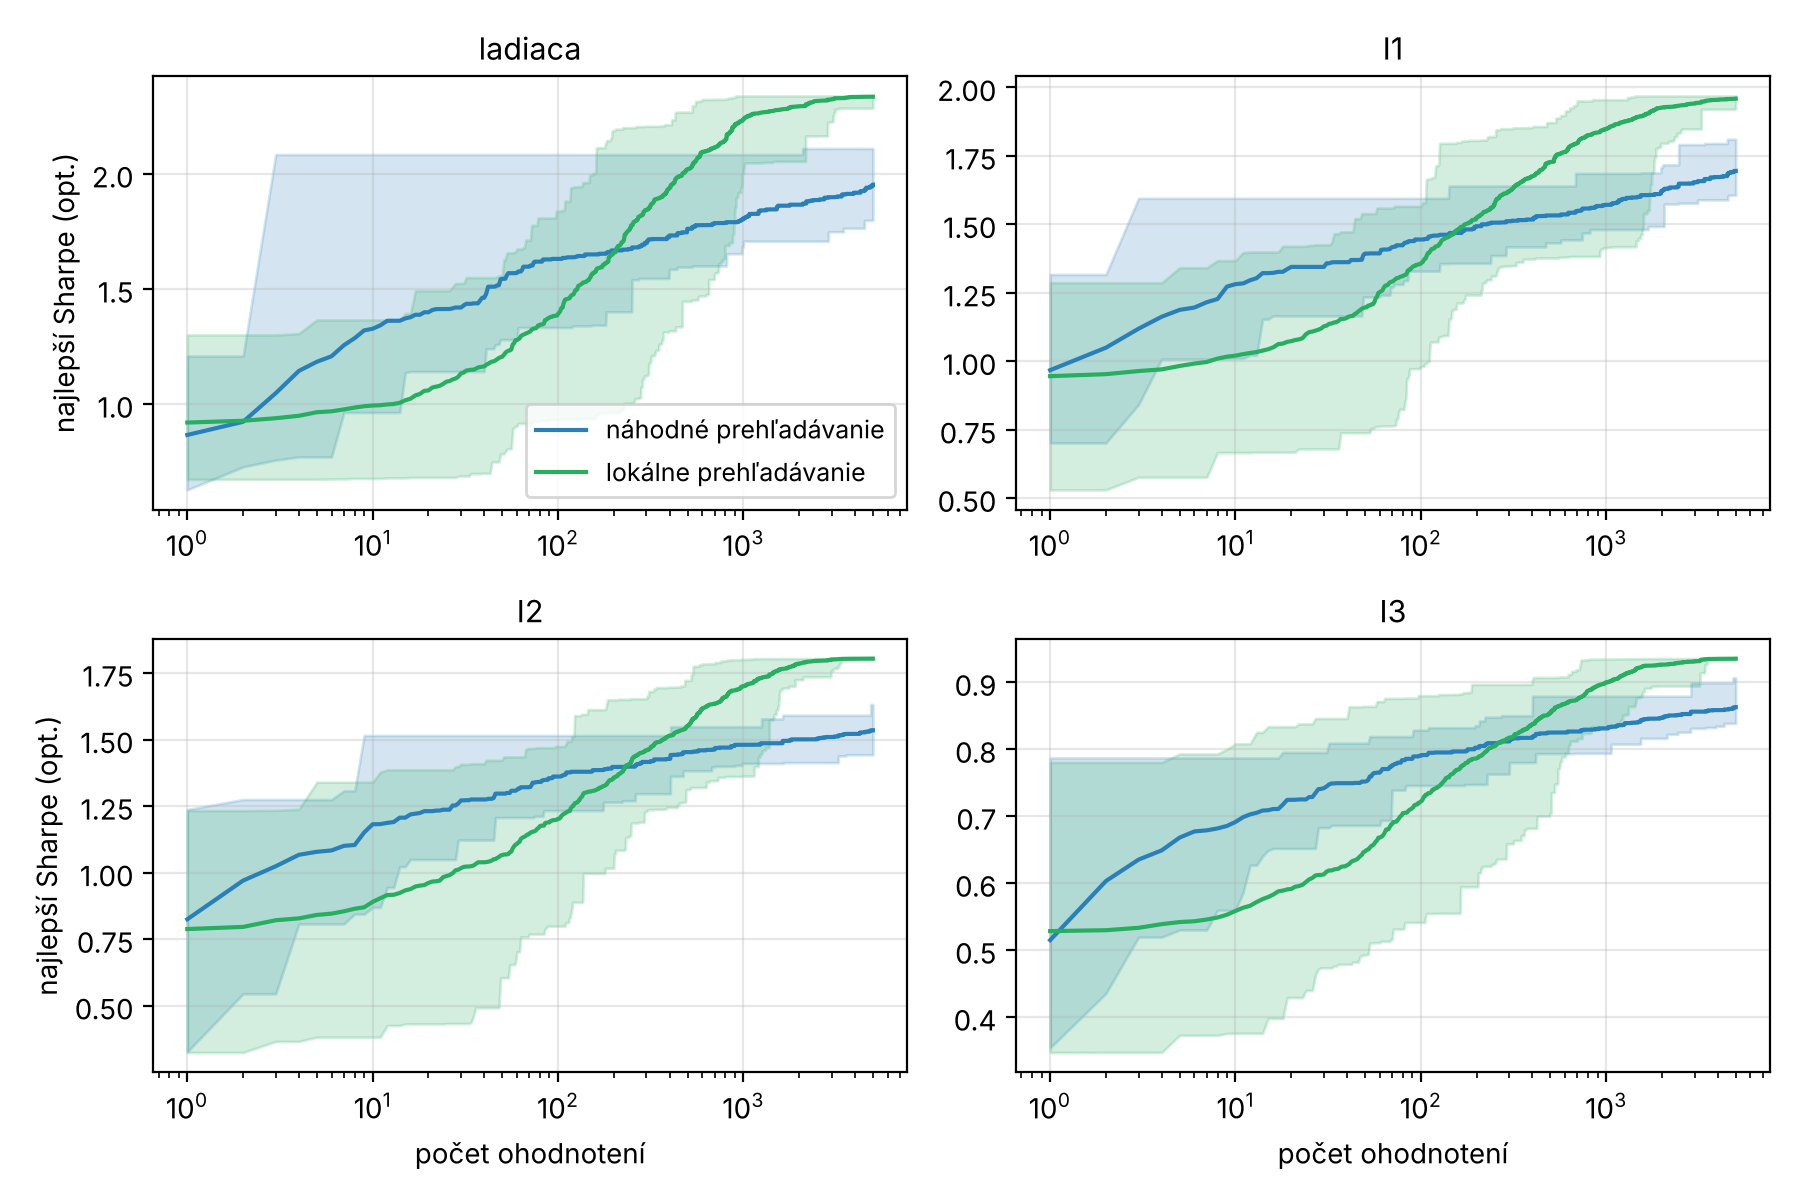
\includegraphics[width=0.8\textwidth]{figures/convergence.png}
\caption{Najlepší Sharpe na optimalizačnom období podľa počtu ohodnotení (priemer cez 20 behov,
pásmo = minimum až maximum).}
\label{fig:conv}
\end{figure}

\paragraph{Čo baseline hovorí o úlohe.} Výsledky sú v~tabuľke~\ref{tab:base}.
\begin{itemize}
\item \textbf{Model aj baseline fungujú}: všetkých 10\,000 náhodných portfólií aj všetky výsledky
  prehľadávaní prešli kontrolou \texttt{check}. Priemerné náhodné portfólio má na teste prakticky
  rovnaký výnos ako 1/N, ale vyššie kolísanie -- 5--10 aktív diverzifikuje horšie ako 30.
\item \textbf{Optimalizácia na optimalizačnom období funguje}: lokálne prehľadávanie zvýši Sharpe
  oproti priemeru náhodných portfólií 1,7- až 2,5-násobne a dostane sa na 1--5\,\% od
  orientačného horného odhadu z~E1. Náhodné prehľadávanie zaostáva a medzi behmi kolíše viac
  (obr.~\ref{fig:conv}). Prvých asi 150--300 ohodnotení je náhodné prehľadávanie lepšie (lokálne
  sa ešte len vzďaľuje od náhodného štartu); konečný výsledok náhodného prehľadávania
  (po 5\,000 ohodnoteniach) prekoná lokálne prehľadávanie v~priemere už po 400--550
  ohodnoteniach a na 1\,\% od svojej konečnej hodnoty sa dostane po 2\,000--3\,000. Pri 30 aktívach je teda úloha na optimalizačnom období
  pomerne ľahká; rozdiely medzi metódami v míľniku 3 budú viditeľnejšie na väčšej úlohe.
\item \textbf{Vyšší Sharpe na minulosti neznamená vyšší Sharpe v budúcnosti.} Korelácia medzi
  obdobiami (obr.~\ref{fig:random}) je v~I1 silná (0,77), v~ladiacej a I3 slabá a v~I2 záporná
  ($-0{,}41$). V~I1 a I3 optimalizácia prekonala náhodné portfóliá aj 1/N aj na teste, v~ladiacej
  inštancii je na úrovni 1/N a v~I2 je výrazne horšia (Sharpe $-0{,}07$, strata 3,4\,\%).
  Príčinou v~I2 je, že v~rokoch 2017--2020 mali najlepší pomer výnosu a kolísania dlhodobé
  dlhopisy a zlato (E1), ktoré potom v~roku 2022 pri rýchlom raste úrokových sadzieb prudko klesli.
  Optimalizácia sa prispôsobila konkrétnej minulosti \cite{michaud1989}. Je to vlastnosť
  ohodnocovacej funkcie (Sharpe na minulosti je len odhad cieľovej funkcie), nie chyba
  algoritmu. Pri porovnaní metód preto budeme oddelene hodnotiť kvalitu optimalizácie
  (Sharpe na optimalizačnom období pri rovnakom rozpočte) a kvalitu výsledku na teste.
\item \textbf{Vyšší Sharpe neznamená vyšší zisk.} Maximalizácia Sharpe uprednostňuje aktíva
  s~nízkym kolísaním (dlhopisy, zlato). V~ladiacej inštancii má lokálne prehľadávanie na teste
  Sharpe na úrovni 1/N, ale ročný výnos len 5,6\,\% oproti 9,4\,\% a konečnú sumu
  11\,776 oproti 13\,082\,USD. Pri porovnaní preto uvádzame aj výnos a konečnú sumu.
\item \textbf{Greedy top-10} zlepší optimalizačné obdobie menej ako prehľadávanie (aktíva s
  vysokým vlastným Sharpe sú často podobné a navzájom korelované). Na teste je v troch
  inštanciách lepší ako priemer náhodných portfólií (v ladiacej najlepší zo všetkých), v~I2 horší.
\end{itemize}

% =====================================================================================
\section{Navrhované metódy pre míľnik 3}
\label{sec:methods}

Skúsenosti z implementácie: ohodnotenie je lacné (desiatky µs), takže si môžeme dovoliť desaťtisíce
ohodnotení na beh a 20--30 behov; obmedzenia vieme vždy splniť opravou za desiatky µs; plocha
vhodnosti v~reprezentácii skóre má plošiny (zmena skóre nevybraného aktíva pod prahom nič nemení),
čo pri lokálnom prehľadávaní rieši prijímanie rovnako dobrých krokov. Úloha má dve vrstvy:
kombinatorický výber aktív a spojité rozdelenie podielov, pričom pre pevný výber je Sharpe
hladká funkcia podielov. Navrhujeme dve zmysluplne odlišné metódy:

\paragraph{1. Genetický algoritmus s priamou reprezentáciou a opravou.} Jedinec je priamo vektor
podielov $w$. Metóda je overená na úlohe s rovnakými pravidlami (počet aktív a minimálny a
maximálny podiel) \cite{chang2000}. Úpravy pre našu úlohu: kríženie zjednotí vybrané aktíva
rodičov a podiely spriemeruje, nadbytočné aktíva odstráni oprava; mutácie
\emph{výmena} (vybrané aktívum nahradí nevybraným so zachovaním podielu), \emph{presun}
(časť podielu z~jedného aktíva na druhé) a \emph{pridanie/odobratie} aktíva; po každej
operácii oprava a opravený jedinec sa vráti do populácie. Turnajový výber, elitizmus, ukončenie
po pevnom počte ohodnotení. Vhodnosť: kríženie môže skladať dobré časti portfólií (napr.
dlhopisovú a akciovú zložku) z rôznych jedincov, čo lokálne prehľadávanie nevie.
Parametre (veľkosť populácie, pravdepodobnosti operátorov) naladíme na ladiacej inštancii.

\paragraph{2. Hybrid: simulované žíhanie nad výberom aktív + presná optimalizácia podielov.}
Úlohu rozdelíme na dve vrstvy. Simulované žíhanie prehľadáva len množiny $S$ s~5--10 aktívami
(susedia: výmena, pridanie, odobratie aktíva). Pre každú množinu $S$ nájde podiely
gradientovým riešiteľom (SLSQP so súčtom 1 a hranicami $[\ell,u]$, štart z~podielov
predchádzajúceho riešenia). Využívame tak, že model je \emph{white-box}: pre pevné $S$ je
úloha hladká a nízkorozmerná ($\le 10$ premenných) a riešiteľ ju vyrieši oveľa presnejšie ako
náhodné zmeny podielov. Úprava pre férovosť: počítame \emph{všetky} ohodnotenia funkcie
vrátane tých vo vnútri riešiteľa (a numerického gradientu), takže metóda má rovnaký rozpočet
ako ostatné; porovnáme aj čas behu. Rizikom je drahý vnútorný krok, preto obmedzíme počet
iterácií riešiteľa a otestujeme aj lacnejšiu verziu, ktorá podiely optimalizuje len pre
najlepšie množiny.

\paragraph{Záloha.} Diferenciálna evolúcia v reprezentácii cez skóre s dekóderom -- pracuje so
spojitými vektormi bez úprav operátorov; použijeme ju, ak by niektorá z metód zlyhala.

\paragraph{Plán experimentov pre míľnik 3.} Všetky metódy (aj náhodné a lokálne prehľadávanie)
spustíme na I1--I3 s rovnakým počtom ohodnotení (5\,000 a 20\,000) a 20--30 nezávislými behmi
s pevnými seedmi. Porovnáme Sharpe na optimalizačnom období (kvalita optimalizácie, odstup od
horného odhadu z~E1), testovacie metriky voči priemeru náhodných portfólií a 1/N, čas behu a
rozptyl medzi behmi; rozdiely overíme Wilcoxonovým testom. Potom úlohu zväčšíme podľa
míľnika 1 (viac aktív, voľnejšie podiely, napr. 60 aktív a $k_{\max}=20$), kde čakáme
väčšie rozdiely medzi metódami.

% =====================================================================================
\section{Obmedzenia a otvorené otázky}
\begin{itemize}
\item Zoznamy 15 najväčších firiem sme zostavili podľa verejných rebríčkov trhovej kapitalizácie
  ku koncu roka; pri firmách s~podobnou veľkosťou môže byť poradie na hranici 15. miesta sporné.
\item Upravené ceny Yahoo Finance predpokladajú okamžité reinvestovanie dividend bez dane;
  poplatky a dane nezapočítavame (rovnako pre všetky metódy).
\item Máme len tri hodnotiace inštancie a tie sa prekrývajú (optimalizačné obdobia sa čiastočne
  kryjú), výsledky na testovacích obdobiach preto nemožno zovšeobecňovať. Silne závisia od
  toho, čo sa v danom období stalo na trhu (napr. rok 2022 pre dlhopisy).
\item Sharpeho pomer počítame bez bezrizikovej sadzby. V~rokoch s~vysokými úrokovými sadzbami
  (napr. 2023--2025) by po jej odpočítaní vyzerali portfóliá s~veľkým podielom dlhopisov horšie,
  takže nulová sadzba ich mierne zvýhodňuje.
\item Výsledky lokálneho prehľadávania sú reprodukovateľné pri rovnakých verziách knižníc
  (\texttt{requirements.txt}); hodnoty $f$ pri porovnávaní zaokrúhľujeme, aby drobné numerické
  rozdiely medzi počítačmi nemenili rozhodnutia na plošinách.
\end{itemize}

\paragraph{Rozdelenie práce.} % TODO doplniť
Lukáš Švihura -- \dots; Dominik Keil -- \dots; Ján Hrbál -- \dots

\begin{thebibliography}{9}
\bibitem{chang2000} T.-J. Chang, N. Meade, J.\,E. Beasley, Y.\,M. Sharaiha.
  Heuristics for cardinality constrained portfolio optimisation.
  \emph{Computers \& Operations Research} 27 (2000), 1271--1302.
\bibitem{demiguel2009} V. DeMiguel, L. Garlappi, R. Uppal.
  Optimal versus naive diversification: How inefficient is the 1/N portfolio strategy?
  \emph{The Review of Financial Studies} 22(5) (2009), 1915--1953.
\bibitem{michaud1989} R.\,O. Michaud. The Markowitz optimization enigma: Is „optimized“ optimal?
  \emph{Financial Analysts Journal} 45(1) (1989), 31--42.
\end{thebibliography}

\end{document}
